\chapter{РАЗРАБОТКА АЛГОРИТМА УПРАВЛЕНИЯ БУФЕРОМ КОМПЕНСАЦИИ ДЖИТТЕРА} \label{chapt1}

Существующие телекоммуникационные системы активно используют различные методы управления: ситуационные, основанные на логике лиц, принимающих решение; автоматические; автоматизированные.
Вместе с тем, за последние годы все более процедур в телекоммуникационных сетях новых поколений осуществляется автоматически, с оптимизацией этих процедур, что позволяет за кратчайшее время получать наибольший эффект от управления данными процедурами.

В существующих технологиях большой удельный вес занимают методы управления основанные на принципах Понселе. Данные принцип основан на предположении о том, что любому обнаруженному возмущению находится адекватное управление, реагирующее на это возмущение.
Структурная схема управления, функционирующая по принципу Понселе, показана на рис. \ref{fig:ponsele}.


\begin{figure}[!h]

\centering
\begin{tikzpicture}
[node distance = 1cm, auto,
% STYLES
every node/.style={node distance=6cm},
% The force style is used to draw the forces' name
force/.style={rectangle, draw, fill=white!10, inner sep=5pt, text width=4cm, text badly centered, minimum height=1.2cm}] 


% Draw forces
\node [force] (resolving) {Принятое решение};
\node [force, right of=resolving] (object) {Управляемый объект};

 \draw [>=latex,->] (resolving) edge node {$u(t)$} (object);
\draw [>=latex,->] (object)    -- +(0,-2)  -| (resolving);
\node (ask) at (3, -2.5) {Подтверждение об исполнении};

\end{tikzpicture} 
\caption{Схема управления по возмущению (принцип Понселе)}
\label{fig:ponsele}
\end{figure}

Логично, что алгоритм компенсации джиттера должен быть реализован на основе подстройки линии задержки, как результат на отклонение оценки задержки. 
Из этого следует, что принцип управления Понселе для синтеза алгоритма управления буфером не подходит. 
Рассмотрим принцип Уатта, который основан на управлении по отклонению.
Данный принцип управления используется в тех устройствах, выходные сигналы которых имеют те или иные отклонения от средних  или типовых значений.
По сути принцип Уатта лежит в основе построения систем автоматического управления. Структурная схема устройства управления, построенного по принципу Уатта, представлена на рис. \ref{fig:uatta}


\begin{figure}[!h]

\centering
\begin{tikzpicture}
[node distance = 1cm, auto,
% STYLES
every node/.style={node distance=3cm},
% The force style is used to draw the forces' name
force/.style={rectangle, draw, fill=white!10, inner sep=5pt, text width=4cm, text badly centered, minimum height=1.2cm}] 


% Draw forces
\node [force] (system) {Управляемая система};
\node [force, below of=resolving] (man) {Устройство управления};
\draw [>=latex,->] (man.180)    -- +(-1,0)  |- node[left] {$u(t)=Y(\Delta x)$} (system.190);

\path[>=latex,->] (system.170){}+(-2,0) edge node {Вход} (system.170);

\path[>=latex,<-] (system.east){}+(2,0) edge node[above] {Выход} (system.east);

\draw[>=latex,->] (system.east){}+(1,0)   |- node[below] {$x\pm\Delta x$} (man.east) ;
%\path[>=latex,->] (system.0) edge node {Выход} (system.0){}+(2,0);


\end{tikzpicture} 
\caption{Схема управления по отклонению (принцип Уатта)}
\label{fig:uatta}
\end{figure}

Методы основанные на данном принципе могут быть реализованы как в централизованном, так и в децинтрализованном варианте.
Их реализация основывается на методах теории оптимального управления, в терминах переменных состояния.
В рамках методов переменных состояния рассматривают два основные вида управления:
\begin{itemize}
 \item управление состоянием системы;
 \item управление наблюдением.
\end{itemize}

Близкие по теоретическим методам, эти виды управлений приводят к различным алгоритмическим решениям.
Назначение этих управлений также различно.

\section{Анализ методов оптимального управления}

\subsection{Управление состоянием системы}

Данный вид управления предназначен для перевода состояния системы из одних фазовых кординат в другие для достижения требуемой структуры или режима сетевого элемента или всей сети в целом. 
Для нахождения нужного управления выбирают критерий оптимальности, в качестве которого обычно используют среднеквадратичных критерий:


\begin{equation}\label{eq41:cko_ted}
J(\vec{x},u)=\frac{1}{2}x^T(t_F)Dx(t_F)+\frac{1}{2}\int^F_0[x^T(t)Qx(t)+u^T(t)Ru(t)]dt,
\end{equation}

\noindent где $t_F$ - финальное время, за которое достигается цель управления. Если система стохастческая, то вместо (\ref{eq41:cko_ted}) используют математическое ожидание критерия:
\begin{equation}\label{eq41:cko_stoh}
M\{J(\vec{x},u)\}\rightarrow \underset{x}{min}.
\end{equation}

Значение управления $u(t)$ находят,  подставляя в (\ref{eq41:cko_ted}) или (\ref{eq41:cko_stoh}) соответствующее уравнение состояния:
\begin{equation}\label{eq41:stat}
\frac{dx(t)}{dt}=Ax(t)+Bu(t)+C\xi(t).
\end{equation}

Поскольку мы имеем дело со случайными процессами, то необходимо использовать критерий (\ref{eq41:cko_stoh}).
При этом, условия теоремы о разделении дают основание вместо переменной $x(t)$ в уравнениях (\ref{eq41:cko_ted}-\ref{eq41:stat}) подставить значения оценки $\hat{x}(t)$ и синтезировать управление по детерминистской схеме.
Структура управления по состоянию системы представлена на рис. \ref{fig:man_stat}.

\begin{figure}[!h]

\centering
\begin{tikzpicture}
[node distance = 1cm, auto,
% STYLES
every node/.style={node distance=3cm},
% The force style is used to draw the forces' name
force/.style={rectangle, draw, fill=white!10, inner sep=5pt, text width=4cm, text badly centered, minimum height=1.2cm}] 


% Draw forces
\node [force] (system) {Управляемая система};
\node [force, below of=resolving] (man) {Управление};
%\node [force, below of=resolving] (man) {Устройство управления};
\node [force] (est) at ($ (man) + (6,0) $) {Оценка};
\draw [>=latex,->] (man.180)    -- +(-1,0)  |- node[left,xshift=1.1cm,yshift=-0.5cm] {$u(t)$} (system.190);

\path[>=latex,->,] (system.170){}+(-2,0) edge node {Вход} (system.170);

\path[>=latex,<-] (system.east){}+(6,0) edge node[above,xshift=2cm] {Выход} (system.east);



\draw[>=latex,->] (system.east) -| (est.north)  ;
\draw[>=latex,->] (est.west) -- node[above] {$\hat{x}(t)$} (man.east)  ;

\end{tikzpicture} 
\caption{Структурная схема управления системы с разделением на отдельные блоки стохастической оценки и детерминированного управления}
\label{fig:man_stat}
\end{figure}

В соответствии с теорией управления, оптимальная траектория, по которой система переводится в требуемое фазовое состояние, определяется при минимизации гамильтона $\EuScript{H}(t)$ вдоль этой траектории:
\begin{equation}\label{eq41:man1}
\frac{d\EuScript{H}(t)}{du}\rightarrow0,
\end{equation}
\noindent где $\EuScript{H}(t)=\frac{1}{2}x^T(t)Qx(t)+\frac{1}{2}u^T(t)Ru(t)+\lambda^T(t)Ax(t)+\lambda^T(t)Bu(t)$.

При выполнении условий (\ref{eq41:man1}) оптимальное управление, соответствующее (\ref{eq41:man1}), находится в виде:
\begin{equation}\label{eq41:man2}
u(t)=R^{-1}B\lambda(t),
\end{equation}

\noindent где $\lambda (t)=D(t_F)x(t_F)$ - приведенное, конечное в момент $t_F$ состояние управляемой системы.
После преобразования для дискретной системы управляющее воздействие имеет вид:

\begin{equation}\label{eq41:man3}
u(k)=L(k,k-1)x(k-1),
\end{equation}
\noindent где $L(k,k-1)=-R^{-1}B^TP(k)$; $P(k)=Q(k)+A^T\lfloor P^{-1}(k-1)+BR^{-1}B\rfloor A.$

Рассмотренное управление носит название терминального или финального, поскольку считается, что после окончания времени $t_F$ управление завершено и система переходит в равновестное состояние.
Однако в нашем случае с помощью управления решается задача поддерживания того или иного состояния джиттера на притяжении довольно длительного времени. 
В этом случае верхний предел интегрирования в \ref{eq41:cko_ted} можно отнести в бесконечность.

Уравнение состояния системы $x(k)$ можно представить в виде:
\begin{equation}\label{eq41:man4}
x(k+1)=e^{-\alpha \Delta t}x(k)+\sqrt{\sigma^2_x(1-e^{-\alpha \Delta t}}\xi(k)+Bu(k),
\end{equation}
\noindent где $\alpha=\tau^{-1}_{cor}$; $\Delta t$ - шаг дискретизации.

Предполагая состояние системы $x(k)$ случайным, решение для критерия (\ref{eq41:cko_ted}) будем находить в соответствии с (\ref{eq41:cko_stoh}), однако при этом придется использовать специальные методы интегрирования стохастических функций.
Более рационально применить условия теоремы о разделении и вместо случайного состояния $x(k)$ использовать его оценку $\hat{x}(k)$. Уравнение (\ref{eq41:man2}) при этом будем находить в виде:
\begin{equation}\label{eq41:man5}
u(k)=-\frac{BP(k)\hat{x}(k)}{R}.
\end{equation}

Представленное выражение для уравнения (\ref{eq41:man5})  включает переходный и установившийся режимы. Для установившегося режима динамика управления зависит лишь от оценки состояния
\begin{equation}\label{eq41:man6}
u(k)=-\frac{BP\hat{x}(k)}{R},
\end{equation}
\noindent где $\hat x (k+1)=e^{-\alpha \Delta t}\hat x(k)+\frac{P}{N_\nu}(y(k)-\hat x(k))$ - оценка дискретного состояния системы (\ref{eq41:man4}).
Точность управления определяется точностью оценки состояния, поскольку в (\ref{eq41:man6}) другие неизвестные параметры и данные не входят.

\subsection{Управление наблюдением системы}

В отличии от управления состоянием управление наблюдением не предполагает каких либо изменений внутренних свойств системы, наоборот - за счет управлений осуществляется преобразование базиса наблюдения.

Рассмотим типовую ситуацию, пусть уравнение наблюдения содержит полезный сигнал $c(t)$, помеху $n(t)$ и белый шум $v(t)$ (рис. \ref{fig:man_1}):

\begin{equation}\label{eq41:man7}
y(t)=c(t)+n(t)+v(t).
\end{equation}

\begin{figure}[!h]

\centering
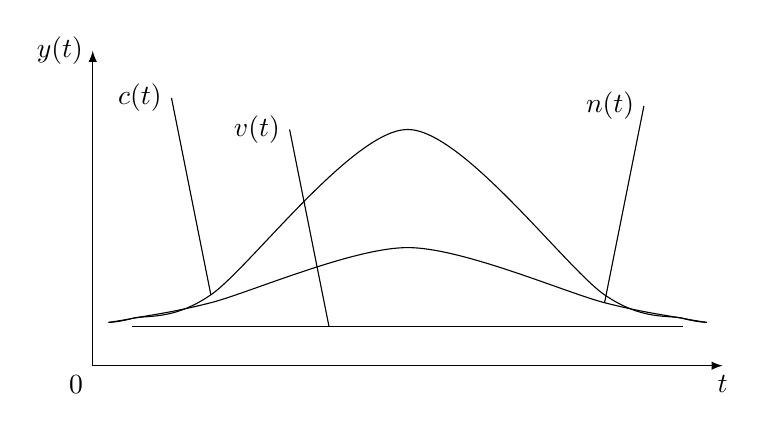
\begin{tikzpicture}

\draw[>=latex,->] (0,0)--(8,0) node[anchor=north] {$t$}; % ось Ox с подписью
\draw[>=latex,->] (0,0)--(0,4) node[anchor=east] {$y(t)$}; % ось Oy с подписью
\draw plot coordinates { (0.5,0.5) (7.5,0.5) };
\draw plot[smooth] coordinates { (0.2,0.55) (0.5,0.6) (1.5,0.9) (4,3) (6.5,0.9) (7.5,0.6) (7.8,0.55) };
\draw plot[smooth] coordinates { (0.2,0.55) (0.5,0.6) (1.5,0.8) (4,1.5) (6.5,0.8) (7.5,0.6) (7.8,0.55) };

\draw plot coordinates { (3,0.5) (2.5,3) } node[anchor=east] {$v(t)$};
\draw plot coordinates { (1.5,0.9) (1,3.4) } node[anchor=east] {$c(t)$};
\draw plot coordinates { (6.5,0.8) (7,3.3) } node[anchor=east] {$n(t)$};
\draw node[anchor=north east] {$0$};


\end{tikzpicture} 
\caption{Наблюдение сигнала с помехой и белым шумом}
\label{fig:man_1}
\end{figure}


Очевидно, что когда уровни полезной составляющей и помеховой составляющей соизмеримы между собой, как это следует из рис. \ref{fig:man_1}, получить удовлетворительное качество оценки затруднительно. 
В этой ситуации уместно использовать адаптивную компенсацию помеховой составляющей $n(t)$.

Необходимо сформировать такой сигнал (антипомеху) $n^*(t)\approx-n(t)$, чтобы вычесть его из наблюдаемой реализации:
\begin{equation}\label{eq41:man8}
y^*(t)=c(t)+n(t)-n^*(t)+v(t)=c(t)+v(t)+\Delta n(t),
\end{equation}
\noindent где $\Delta n(t)$ - остаток нескомпенсированной помеховой составляющей, который следует минимизировать: $\Delta n(t)\longrightarrow 0$.

Однако формированию <<антипомехи>> $n^*(t)$ из основного источника наблюдения (\ref{eq41:man7}) мешает полезная составляющая $c(t)$, уровень, которой может быть значительным (рис. \ref{fig:man_1}).
Таким образом, прямого решения нет.
В связи с этим, задача компенсации расширяется и реализовывается в два этапа: в начале находится возможность создания <<антипомехи>>, а потом скомпенсировать в помеху в наблюдении.


\section{Метод управления наблюдением для реализации буфера компенсации джиттера}

Как упоминалось ранее, из теории автоматического управления известна теорема о разделении \cite{seij, red}, утверждающая о том, что при среднеквадратичном критерии качества и
при гауссовской ситуации, оптимальное управнение можно построить из двух раздельных процедур: оптимальной стохастической оценки $\hat x (k)$  и детерминированной процедуры управления:
\begin{equation}\label{eq41:man9}
u(t)=\EuScript{L}(k)\hat x (k),
\end{equation}

Воспользуемся результатами данной теоремы.

Прежде, чем приступить к синтезу алгоритмов управления, следует уточнить, каким способом будет осуществлятся управление буфером компесации джиттера поступающих пакетов. 
Очевидно, это может быть реализованно с помощью аддитивной коррекции:
\begin{equation}\label{eq41:man10}
y(k)\pm\hat x(k)
\end{equation}
или мультипликативной коррекции:
\begin{equation}\label{eq41:man11}
y(k)(l\hat x(k)),
\end{equation}
\noindent где $l$ - масштабирующий множетель.

Для разработки алгоритмов управления воспользуемся процедурой ФКБ (\ref{eq3:Estim_rel}). Очевидно, для решения задачи необходимо выбрать вариант управления наблюдением (\ref{eq41:man8}),
поскольку именно наблюдаемую величину необходимо корректировать, выбирая или оценивая соответствующую величину коэффициента $H(k)$. 
В литературе \cite{windrow,monzigo} процедуры оценки весовых коэффициентов известны как адаптивные алгоритмы Уидроу-Хоффа. 
Следуя данной литературе переобозначим $H(k)\equiv W(k)$ и будем находить оптимальную оценку этого коэффициента на основании уравнения (\ref{eq3:Estim_rel}):
\begin{equation}\label{eq41:man12}
\hat W(k+1)=\hat W(k)+K(k)[y(k)-\hat W(k)y_{g}]y_{g},
\end{equation}

Весовой коэффициент $\hat W(k)$ может быть как вещественным, так и комплексным. 
В первом случае буфер компенсации джиттера обеспечивает процедуру в соответствии с (\ref{eq41:man10}). 
Структурная схема устройства управления, реализующего алгоритм (\ref{eq41:man12}), представлена на рис. \ref{fig:man_2}
